\chapter{Chemische boodschappers en signaaltransductie}\label{ch:b2:cell-signalling}

Eén enkel molecuul adrenaline dat aan het oppervlak van een levercel
aankomt, gaat die cel nooit binnen. Het bindt aan een eiwit aan de
buitenkant, verandert de vorm van dat eiwit, en binnen een seconde heeft
de cel tienduizend moleculen van een \omterm{prop:b2:cell-signalling:gpcr}{secundaire boodschapper} gemaakt,
honderdduizend enzymmoleculen geactiveerd en is ze begonnen een miljoen
moleculen glucose vrij te geven --- een keten van versterkingen van een
factor miljoen, in gang gezet door een signaal dat buiten de deur bleef. Dit
hoofdstuk gaat over de boodschappers die cellen elkaar sturen en over hoe een
cel een boodschap aan haar oppervlak omzet in een verandering van haar
chemie, haar genen of haar vorm: de receptoren, de \omterm{prop:b2:cell-signalling:gpcr}{secundaire
boodschappers}, de cascades van kinasen, en de twee ontwerpen --- de snelle,
bedrade signalering van zenuwen en de trage, uitgezonden signalering van
hormonen --- waarvan het contrast door de rest van dit boek loopt.

\section{Boodschappers}

\begin{definition}[Soorten chemische signalering]\label{def:b2:cell-signalling:kinds}
\index{hormoon}\index{endocriene signalering}\index{paracriene signalering}\index{neurotransmitter}
Een cel geeft een signaal aan een andere met een uitgescheiden molecuul, een
\emph{boodschapper} of \emph{ligand}, dat bindt aan een \emph{receptor} op
of in het doelwit. Naar bereik: \emph{endocriene} signalering, waarbij een
\emph{hormoon} door een klier in het \omterm{def:b2:blood-circulation:blood}{bloed} wordt afgegeven en elke cel van
het lichaam bereikt, maar alleen inwerkt op cellen met de receptor, over
minuten tot uren (insuline, cortisol, adrenaline, thyroxine);
\emph{paracriene} signalering, waarbij de boodschapper naar naburige cellen
binnen een millimeter diffundeert en onderweg wordt afgebroken
(groeifactoren, histamine, prostaglandinen, de morfogenen van
\cref{ch:b2:vertebrate-development}); \emph{autocriene} signalering, waarbij
de cel een signaal aan zichzelf geeft; en \emph{synaptische}, waarbij een
neuron een \emph{neurotransmitter} over een spleet van \qty{20}{nm} op één
doelcel afgeeft, in een milliseconde (\cref{ch:b2:neurons-synapses}).
Naar chemie: \emph{wateroplosbare} boodschappers --- aminozuurderivaten
zoals adrenaline, peptiden en eiwitten zoals insuline --- kunnen het membraan
niet passeren en werken in op receptoren aan het oppervlak;
\emph{vetoplosbare} boodschappers --- de steroïden (cortisol, oestradiol,
testosteron), thyroxine, retinoïnezuur, stikstofmonoxide --- passeren het wel
en werken in op receptoren binnenin. Het endocriene stelsel en het zenuwstelsel
zijn de twee manieren waarop een lichaam van $10^{13}$ cellen zichzelf
coördineert: het ene zendt traag naar iedereen uit, het andere legt snel
een draad naar iemand.
\end{definition}

\begin{omfigure}
\begin{tikzpicture}[every node/.style={font=\scriptsize}, >=stealth]
  % endocrine
  \begin{scope}
    \draw[thick, fill=omProp!25] (0,1.6) circle (0.35); \node[above] at (0,2.0) {klier};
    \draw[very thick, omThm!60] (-0.5,0.6) -- (4.5,0.6); \draw[very thick, omThm!60] (-0.5,0.2) -- (4.5,0.2); \node[omThm!70!black] at (2,0.4) {bloed};
    \foreach \x in {0.6,1.5,2.4,3.3} \fill[omProp] (\x,0.4) circle (0.05);
    \draw[->, omProp] (0,1.25) -- (0,0.65);
    \draw[thick, fill=omDef!20] (3.8,-0.8) circle (0.35); \node[below, align=center] at (3.8,-1.2) {doelcel\\met receptor};
    \draw[->, omProp] (3.8,0.15) -- (3.8,-0.4);
    \draw[thick, fill=gray!20] (1.0,-0.8) circle (0.35); \node[below, align=center] at (1.0,-1.2) {geen receptor:\\negeert het};
    \node[align=center] at (2.2,-2.4) {endocrien: hormoon in het bloed,\\hele lichaam, minuten tot uren};
  \end{scope}
  % paracrine
  \begin{scope}[xshift=6.6cm]
    \draw[thick, fill=omProp!25] (0.8,0.6) circle (0.35);
    \foreach \a in {0,45,...,315} \fill[omProp] (0.8,0.6) ++(\a:0.6) circle (0.04);
    \draw[thick, fill=omDef!20] (1.9,0.9) circle (0.3); \draw[thick, fill=omDef!20] (1.7,-0.2) circle (0.3); \draw[thick, fill=omDef!20] (-0.2,0.0) circle (0.3);
    \node[align=center] at (0.8,-2.4) {paracrien: diffundeert naar\\buren, afgebroken\\binnen een millimeter};
  \end{scope}
  % synaptic
  \begin{scope}[xshift=11.6cm]
    \draw[very thick, omDef] (0,1.8) -- (0,0.5); \draw[thick, fill=omDef!25] (0,0.3) circle (0.25);
    \draw[thick, fill=omExo!30] (0,-0.5) circle (0.3);
    \foreach \x in {-0.08,0,0.08} \fill[omProp] (\x,-0.05) circle (0.03);
    \node[align=center] at (0.2,-2.4) {synaptisch: één doelwit,\\\qty{20}{nm},\\een milliseconde};
  \end{scope}
\end{tikzpicture}

{\small Drie bereiken van chemische signalering: een \omterm{def:b2:cell-signalling:kinds}{hormoon} dat door het
\omterm{def:b2:blood-circulation:blood}{bloed} naar elke cel met zijn receptor wordt uitgezonden; een paracriene
factor die zijn buren bereikt; een \omterm{def:b2:cell-signalling:kinds}{neurotransmitter} die via een synaps aan
één cel wordt afgeleverd.}
\end{omfigure}

\begin{theorem}[Receptorbezetting]\label{thm:b2:cell-signalling:occupancy}
\index{dissociatieconstante}\index{receptorbezetting}
Een receptor $R$ bindt zijn ligand $L$ omkeerbaar, $R + L
\rightleftharpoons RL$, met een \emph{\omterm{thm:b2:cell-signalling:occupancy}{dissociatieconstante}} $K_d =
[R][L]/[RL]$. In evenwicht is de fractie bezette receptoren
\[
\theta = \frac{[RL]}{[R]_{\text{tot}}} = \frac{[L]}{K_d + [L]},
\]
dezelfde hyperbool als de verzadiging van een enzym. $K_d$ is de
concentratie waarbij de helft van de receptoren bezet is, en meet de
\emph{affiniteit}: hoe lager, hoe steviger. Hormoonreceptoren hebben een
$K_d$ in het nanomolaire tot picomolaire bereik, afgestemd op de
concentraties waarin hormonen circuleren ($10^{-12}$ tot
$10^{-9}$ mol/L): bij $[L] = K_d/10$ is een tiende bezet, bij
$10K_d$ negen tiende. Een cel kan niet reageren op een \omterm{def:b2:cell-signalling:kinds}{hormoon} waarvoor ze
geen receptoren heeft, en ze stemt haar gevoeligheid af door het aantal
receptoren te veranderen, of --- zoals in \cref{ch:b2:reproductive-hormones}
--- door ze in te trekken wanneer het \omterm{def:b2:cell-signalling:kinds}{hormoon} voortdurend aanwezig is.
\end{theorem}
\begin{proof}
Met $[R] = [R]_{\text{tot}} - [RL]$ is $K_d = ([R]_{\text{tot}} -
[RL])[L]/[RL]$, dus $[RL](K_d + [L]) = [R]_{\text{tot}}[L]$, wat de
formule is. Het is de uitdrukking van Michaelis--Menten uit het deel van
jaar 1 zonder de katalytische stap.
\end{proof}

\begin{omfigure}
\begin{tikzpicture}
\begin{axis}[
  width=0.68\linewidth, height=5.2cm,
  axis x line=bottom, axis y line=left,
  xmode=log, xmin=0.01, xmax=100, ymin=0, ymax=1.1,
  xlabel={ligandconcentratie (eenheden $K_d$)}, ylabel={fractie bezette receptoren},
  xlabel style={font=\small, at={(axis description cs:0.5,-0.13)}, anchor=north},
  ylabel style={font=\small},
  tick label style={font=\small}, xtick={0.01,0.1,1,10,100}, ytick={0,0.5,1},
  clip=false,
]
\addplot[very thick, omDef, domain=0.01:100, samples=100] {x/(1+x)};
\draw[dashed, gray] (axis cs:1,0) -- (axis cs:1,0.5) -- (axis cs:0.01,0.5);
\node[font=\scriptsize, anchor=north west] at (axis cs:1.1,0.48) {$[L] = K_d$: half bezet};
\node[font=\scriptsize, anchor=south east] at (axis cs:0.1,0.1) {10\% bij $K_d/10$};
\node[font=\scriptsize, anchor=north west] at (axis cs:10,0.92) {90\% bij $10\,K_d$};
\end{axis}
\end{tikzpicture}

{\small \omterm{thm:b2:cell-signalling:occupancy}{Receptorbezetting} tegen ligandconcentratie op een logaritmische
schaal: de respons van een cel loopt van een tiende tot negen tiende over
een honderdvoudig concentratiebereik rond $K_d$.}
\end{omfigure}

\section{Receptoren aan het oppervlak}

\begin{proposition}[G-eiwitgekoppelde receptoren en cyclisch AMP]\label{prop:b2:cell-signalling:gpcr}
\index{G-eiwit}\index{G-eiwitgekoppelde receptor}\index{cyclisch AMP}\index{secundaire boodschapper}\index{proteïnekinase A}
De grootste familie van receptoren --- zo'n \num{800} genen bij de mens,
voor hormonen, \omterm{def:b2:cell-signalling:kinds}{neurotransmitters}, geuren, licht --- bestaat uit eiwitten die
het membraan zeven keer doorkruisen. Een ligand dat buiten bindt, verandert
hun vorm binnen, waar ze een \emph{G-eiwit} activeren: een schakelaar van
drie subeenheden die zijn gebonden GDP voor GTP verwisselt, uiteenvalt, en
in zijn GTP-gebonden vorm enkele seconden een effectorenzym regelt, voordat
het GTP hydrolyseert en zichzelf uitschakelt. De klassieke effector is
\emph{adenylaatcyclase}, dat uit ATP \emph{\omterm{prop:b2:cell-signalling:gpcr}{cyclisch AMP}} maakt: een kleine,
diffundeerbare \emph{\omterm{prop:b2:cell-signalling:gpcr}{secundaire boodschapper}} waarvan de concentratie binnen
seconden stijgt van \qty{0.1}{\micro mol/L} tot enkele micromolair, en die
\emph{\omterm{prop:b2:cell-signalling:gpcr}{proteïnekinase A}} activeert, een enzym dat tientallen doeleiwitten
fosforyleert --- en ze zo aan- of uitschakelt. Het signaal wordt beëindigd
door fosfodiësterase, dat cAMP afbreekt, en door fosfatasen, die de
fosfaatgroepen verwijderen. Adrenaline werkt zo op een levercel: receptor
$\to$ G-eiwit
$\to$ cyclase $\to$ cAMP $\to$ kinase A $\to$ fosforylasekinase
$\to$ glycogeenfosforylase $\to$ glucose. Glucagon gebruikt dezelfde route;
andere G-eiwitten remmen het cyclase, of activeren fosfolipase C, dat twee
andere \omterm{prop:b2:cell-signalling:gpcr}{secundaire boodschappers} vrijmaakt, \emph{inositoltrisfosfaat} ---
dat calciumvoorraden opent --- en diacylglycerol.
\end{proposition}
\begin{proof}[Bewijsmateriaal]
Sutherland (1957) toonde aan dat adrenaline die aan een homogenaat van lever
werd toegevoegd, alleen glucose vrijmaakte als er membranen aanwezig waren,
dat de membranen een hittestabiele factor maakten die op zichzelf het
fosforylase in de membraanvrije fractie activeerde, en dat die factor
\omterm{prop:b2:cell-signalling:gpcr}{cyclisch AMP} was --- de eerste \omterm{prop:b2:cell-signalling:gpcr}{secundaire boodschapper}, en het eerste bewijs
dat een \omterm{def:b2:cell-signalling:kinds}{hormoon} aan het celoppervlak werkt via een intracellulaire
tussenstof. Rodbell en Gilman (jaren 1970) vonden dat het cyclase GTP nodig
had en isoleerden het G-eiwit dat het signaal tussen receptor en enzym
overbrengt; choleratoxine, dat het G-eiwit in zijn aan-toestand vastzet,
laat de darm liters vocht per dag afscheiden --- de ziekte is een defect van
de signalering.
\end{proof}

\begin{omfigure}
\begin{tikzpicture}[every node/.style={font=\scriptsize}, >=stealth]
  % membrane
  \fill[omExo!30] (0,2.0) rectangle (12,2.5);
  \node[anchor=east] at (-0.1,2.25) {membraan};
  % receptor
  \draw[thick, fill=omDef!40] (1.0,1.7) rectangle (1.8,2.8); \node[anchor=east] at (0.95,2.65) {receptor};
  \fill[omProp] (1.4,3.35) circle (0.12); \node[omProp, above] at (1.4,3.45) {adrenaline};
  \draw[->, omProp] (1.4,3.23) -- (1.4,2.85);
  % G protein
  \draw[thick, fill=omDef!25] (2.6,1.5) ellipse (0.72 and 0.36); \node at (2.6,1.5) {G-eiwit};
  \node[below] at (2.6,1.1) {GDP $\to$ GTP};
  \draw[->, thick] (1.8,2.0) -- (2.2,1.75);
  % cyclase
  \draw[thick, fill=omDef!40] (4.2,1.7) rectangle (5.2,2.8); \node[above] at (4.7,2.85) {adenylaatcyclase};
  \draw[->, thick] (3.15,1.5) -- (4.2,1.85);
  % cAMP
  \node[omThm, anchor=west] at (5.35,1.55) {ATP $\to$ cAMP};
  \draw[->, thick, omThm] (4.7,1.7) -- (5.2,1.15);
  % PKA
  \draw[thick, fill=omThm!20] (7.3,0.9) ellipse (0.7 and 0.35); \node at (7.3,0.9) {kinase A};
  \draw[->, thick, omThm] (6.4,0.9) -- (6.6,0.9);
  % targets
  \draw[->, thick] (8.0,0.9) -- (9.0,0.9);
  \node[anchor=west, align=left] at (9.0,0.9) {fosforylasekinase $\to$ fosforylase\\$\to$ glycogeen $\to$ glucose};
  % amplification annotations
  \node[gray, align=center] at (1.4,0.3) {1 hormoon};
  \node[gray, align=center] at (4.7,0.3) {$\sim 10^{2}$ G-eiwitten};
  \node[gray, align=center] at (7.3,0.3) {$\sim 10^{4}$ cAMP};
  \node[gray, align=center] at (10.2,0.3) {$\sim 10^{6}$ glucose};
  % off switches
  \node[omExo!70!black, align=center, anchor=south] at (9.6,2.7) {uit: hydrolyse van GTP (seconden),\\fosfodiësterase breekt cAMP af,\\fosfatasen maken de fosforyleringen ongedaan};
\end{tikzpicture}

{\small De cAMP-route van adrenaline naar glucose. Elk stadium activeert veel
kopieën van het volgende: één hormoonmolecuul eindigt in een miljoen
moleculen product.}
\end{omfigure}

\begin{theorem}[Versterking in een cascade]\label{thm:b2:cell-signalling:amplification}
\index{versterking (signalering)}
Als elk van $n$ stadia van een cascade tijdens de levensduur van zijn eigen
activering $a$ moleculen van het volgende activeert, levert één molecuul
boodschapper $a^{n}$ moleculen eindproduct op. Met vier versterkende stadia
van elk honderd --- een receptor die honderd G-eiwitten activeert, een
cyclase dat honderd cAMP maakt, een kinase dat honderd enzymen fosforyleert,
een enzym dat honderd glucosemoleculen vrijmaakt --- is $a^{n} = 10^{8}$; in
de praktijk een miljoen of zo, in enkele seconden, uit een \omterm{def:b2:cell-signalling:kinds}{hormoon} van
$10^{-9}$ mol/L. Versterking is de reden waarom hormonen werkzaam kunnen zijn
bij concentraties die een miljoen keer lager liggen dan die van de
metabolieten die ze sturen, en waarom de cascade in elk stadium moet worden
uitgeschakeld: een versterker die niet uit kan, is een ziekte (cholera, en de
vele kankers waarin een signaaleiwit in de aan-stand vastzit).
\end{theorem}
\begin{proof}
Stadium 1 levert $a$ actieve moleculen; elk daarvan levert er $a$
in stadium 2, wat $a^{2}$ geeft; door inductie $a^{n}$ na $n$ stadia.
De versterking van elk stadium is het aantal substraatomzettingen dat een
geactiveerde katalysator bereikt voordat hij wordt geïnactiveerd: zijn
katalytische snelheid maal zijn actieve levensduur.
\end{proof}

\begin{proposition}[Receptortyrosinekinasen en calcium]\label{prop:b2:cell-signalling:rtk}
\index{receptortyrosinekinase}\index{insulinereceptor}\index{calciumsignalering}\index{calmoduline}
Een tweede familie van oppervlaktereceptoren --- voor insuline, voor de
groeifactoren die de celdeling aandrijven, voor de inductieve signalen van de
ontwikkeling --- bestaat uit \emph{\omterm{prop:b2:cell-signalling:rtk}{receptortyrosinekinasen}}: eiwitten die het
membraan één keer doorkruisen en die, wanneer hun ligand er twee samenbrengt,
elkaar op tyrosines fosforyleren en zo aanlegplaatsen scheppen voor een reeks
adaptoreiwitten. Van daaruit lopen tegelijk meerdere cascades: een keten van
drie kinasen (de MAP-kinasecascade) die in de kern eindigt en de genen van
de groei aanschakelt; een lipidekinase waarvan het product het kinase
rekruteert dat de metabole effecten van insuline tot stand brengt ---
glucosetransporters naar het membraan verplaatsen, de glycogeensynthese
aanschakelen; en andere. Een derde universele \omterm{prop:b2:cell-signalling:gpcr}{secundaire boodschapper} is
\emph{calcium}: in het cytosol op \qty{0.1}{\micro mol/L} gehouden, tienduizend
keer lager dan buiten, stroomt het binnen via kanalen die door een signaal
of een spanning worden geopend, of komt het uit het endoplasmatisch
reticulum als antwoord op inositoltrisfosfaat, en stijgt het in
milliseconden tot micromolair; gebonden aan \emph{calmoduline} activeert het
kinasen en pompen, en gebonden aan troponine zet het de samentrekking in gang
(\cref{ch:b2:muscle-movement}). Pompen brengen het binnen een seconde terug
naar de voorraden. Welke receptor het ook is, het inwendige van de cel spreekt
maar een paar talen --- cAMP, calcium, fosforylering --- en de specificiteit
ligt in welke eiwitten elk celtype heeft om ze op te laten inwerken.
\end{proposition}

\begin{omfigure}
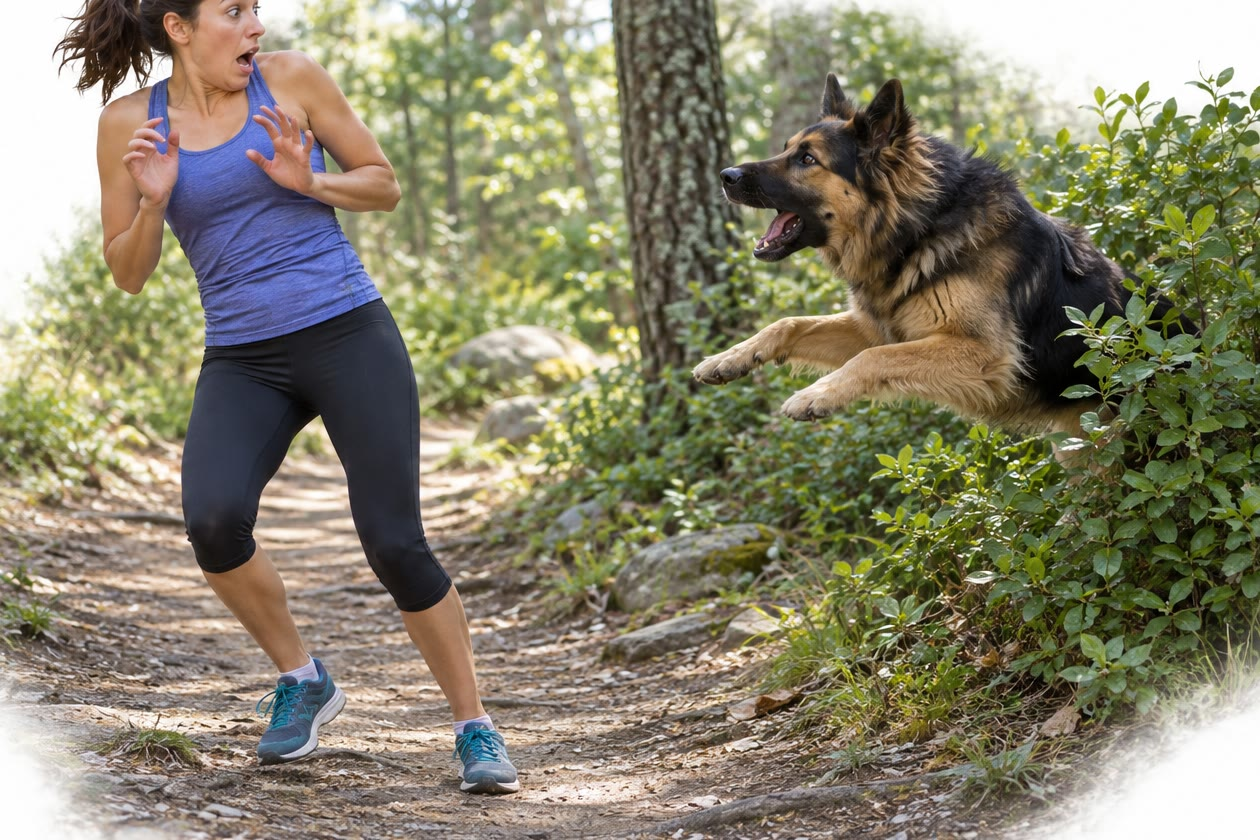
\includegraphics[width=0.6\linewidth]{images/book4/ai/b4-19-adrenaline-runner.jpg}

{\small De cascade aan het werk. Een schrik doet het bijniermerg adrenaline
afgeven; binnen seconden gaat het \omterm{def:b2:heart:anatomy}{hart} tekeer, stort de lever glucose uit
en verwijden de luchtwegen --- één boodschapper, meerdere receptoren, een
versterking van een factor miljoen in elke cel.}
\end{omfigure}

\section{Receptoren binnenin}

\begin{proposition}[Kernreceptoren]\label{prop:b2:cell-signalling:nuclear}
\index{kernreceptor}\index{steroïdhormoon}
Steroïden, thyroxine, retinoïnezuur en vitamine D diffunderen door het
membraan en binden receptoren in het cytosol of de kern die zelf
\emph{\omterm{prop:b2:cell-differentiation:transcriptional}{transcriptiefactoren}} zijn: het complex van \omterm{def:b2:cell-signalling:kinds}{hormoon} en receptor bindt
specifieke DNA-sequenties en schakelt zijn doelgenen aan of uit. De respons
is traag --- minuten tot uren om het mRNA en het eiwit te maken --- en
blijvend: cortisol induceert urenlang de enzymen van de gluconeogenese,
oestradiol bouwt in enkele dagen het baarmoederslijmvlies op, testosteron
maakt in weken spier, thyroxine bepaalt het metabolisme van elke cel. Sommige
steroïden hebben ook snelle effecten via oppervlaktereceptoren, en sommige
oppervlakteroutes bereiken ook de kern (de MAP-kinasecascade), zodat het
onderscheid niet absoluut is; maar de regel blijft dat een vetoplosbare
boodschapper verandert wat een cel \emph{is} door haar genen te veranderen,
terwijl een wateroplosbare verandert wat ze \emph{doet} door haar enzymen te
veranderen.
\end{proposition}

\begin{omfigure}
\begin{tikzpicture}[every node/.style={font=\scriptsize}, >=stealth]
  \foreach \x/\t in {0/{wateroplosbaar: adrenaline, insuline, glucagon}, 7.4/{vetoplosbaar: cortisol, oestradiol, thyroxine}} \node[anchor=south, font=\scriptsize\bfseries] at (\x+2.6,3.4) {\t};
  % left: surface receptor
  \fill[omExo!30] (0,2.4) rectangle (5.2,2.8);
  \draw[thick, fill=omDef!40] (1.6,2.1) rectangle (2.3,3.1);
  \fill[omProp] (1.95,3.35) circle (0.1);
  \draw[->, thick] (1.95,2.1) -- (1.95,1.6) node[below, align=center] {secundaire boodschappers,\\kinasen: enzymen\\in seconden geschakeld};
  \node[align=center] at (4.5,1.0) {verandert wat\\de cel doet};
  % right: nuclear receptor
  \begin{scope}[xshift=7.4cm]
    \fill[omExo!30] (0,2.4) rectangle (5.2,2.8);
    \fill[omProp] (1.5,3.35) circle (0.1);
    \draw[->, omProp] (1.5,3.25) -- (1.5,1.9);
    \draw[thick, fill=omThm!20] (1.5,1.5) ellipse (0.72 and 0.3); \node at (1.5,1.5) {receptor};
    \draw[thick] (0.6,0.4) -- (4.6,0.4); \draw[thick] (0.6,0.25) -- (4.6,0.25); \node[below] at (2.6,0.2) {DNA: doelgenen aan of uit, uren};
    \draw[->, thick] (1.5,1.2) -- (2.4,0.5);
    \node[align=center] at (4.0,1.4) {verandert wat\\de cel is};
  \end{scope}
\end{tikzpicture}

{\small Twee ontwerpen. Een wateroplosbare boodschapper werkt aan het
oppervlak en verandert binnen seconden de enzymactiviteit; een vetoplosbare
gaat naar binnen, bindt een receptor die een \omterm{prop:b2:cell-differentiation:transcriptional}{transcriptiefactor} is, en
verandert over uren de genexpressie.}
\end{omfigure}

\section{Een uitgewerkt voorbeeld: insuline, glucagon en de instelwaarde van glucose}

\begin{proposition}[Twee hormonen en een instelwaarde]\label{prop:b2:cell-signalling:glucose}
\index{insuline}\index{glucagon}\index{bloedglucose}
De glucose in het \omterm{def:b2:blood-circulation:blood}{bloed} wordt rond \qty{5}{mmol/L} (\qty{0.9}{g/L}) gehouden
door twee antagonistische hormonen van de eilandjes van de alvleesklier. Na
een maaltijd wordt de stijgende glucose waargenomen door de $\beta$-cellen ---
die haar metaboliseren, een kaliumkanaal sluiten naarmate hun ATP stijgt,
depolariseren, calcium binnenlaten en \emph{insuline} vrijgeven --- en
insuline laat, via haar tyrosinekinasereceptor, spier- en vetweefsel glucose
opnemen (door transporters naar hun membranen te verplaatsen), de lever haar
als glycogeen en vet opslaan, en alle weefsels ophouden met vet verbranden.
Tussen de maaltijden laat de dalende glucose de $\alpha$-cellen
\emph{glucagon} vrijgeven, dat via cAMP in de lever glycogeen afbreekt en uit
aminozuren nieuwe glucose maakt; adrenaline doet hetzelfde sneller in
noodsituaties, en cortisol en groeihormoon over uren. Elk \omterm{def:b2:cell-signalling:kinds}{hormoon} wordt
vrijgegeven naar verhouding van de afwijking die het corrigeert: een negatieve
terugkoppeling met twee effectoren, één voor elke richting, en een
instelwaarde die tot op een vijfde wordt verdedigd. De hersenen, die
\qty{120}{g} glucose per dag verbranden en er niets van opslaan, zijn het
orgaan dat de lus beschermt; diabetes type 1 is het verlies van de
$\beta$-cellen, en het onbehandelde verloop ervan --- glucose op
\qty{20}{mmol/L}, vet verbrand bij gebrek aan insuline, zuur in het \omterm{def:b2:blood-circulation:blood}{bloed}
--- is hoe de lus eruitziet als één arm is weggenomen.
\end{proposition}

\begin{omfigure}
\begin{tikzpicture}
\begin{axis}[
  width=0.82\linewidth, height=5.6cm,
  axis x line=bottom, axis y line=left,
  xmin=0, xmax=6, ymin=0, ymax=1.1,
  xlabel={uren na een maaltijd}, ylabel={relatief t.o.v.\ piek},
  xlabel style={font=\small, at={(axis description cs:0.5,-0.12)}, anchor=north},
  ylabel style={font=\small},
  tick label style={font=\small}, xtick={0,1,2,3,4,5,6}, ytick={0,0.5,1},
  legend style={font=\scriptsize, at={(0.5,-0.28)}, anchor=north, draw=none, legend columns=3},
  clip=false,
]
\addplot[very thick, omDef, domain=0:6, samples=80] {0.55 + 0.45*exp(-((x-0.9)^2)/0.5) - 0.08*exp(-((x-4)^2)/2)};
\addlegendentry{bloedglucose (5 mmol/L bij 0.55)}
\addplot[very thick, omThm, domain=0:6, samples=80] {0.15 + 0.85*exp(-((x-1.1)^2)/0.45)};
\addlegendentry{insuline}
\addplot[very thick, omProp, domain=0:6, samples=80] {0.75 - 0.5*exp(-((x-1.2)^2)/0.8) + 0.25*(1-exp(-x/5))*0.6};
\addlegendentry{glucagon}
\end{axis}
\end{tikzpicture}

{\small Glucose, insuline en glucagon na een maaltijd. Insuline stijgt met de
glucose mee en brengt haar omlaag; terwijl de glucose naar de instelwaarde
daalt, stijgt glucagon om haar daar te houden.}
\end{omfigure}

\begin{example}[Snelheid, bereik en kosten van de twee systemen]\label{ex:b2:cell-signalling:compare}
Adrenaline in het \omterm{def:b2:blood-circulation:blood}{bloed} bereikt elke cel in ongeveer een minuut (de
circulatietijd) en werkt minutenlang; een zenuwimpuls bereikt zijn doelwit in
milliseconden en werkt milliseconden. Een \omterm{def:b2:cell-signalling:kinds}{hormoon} kost bijna niets per
bereikte cel --- een nanomol verspreid over het lichaam --- maar kan geen
enkele cel afzonderlijk aanspreken; een zenuw spreekt precies één cel aan,
maar moet er een draad naartoe bouwen en onderhouden. Het lichaam gebruikt
beide: de sympathische zenuwen van \cref{ch:b2:blood-pressure} werken in een
seconde op het \omterm{def:b2:heart:anatomy}{hart} en de \omterm{def:b2:blood-circulation:vessels}{arteriolen} in, en het bijniermerg, zelf een
gewijzigde sympathische zenuwknoop, ondersteunt ze door hetzelfde molecuul
voor het hele lichaam in het \omterm{def:b2:blood-circulation:blood}{bloed} te storten. En in de synaps komen de twee
ontwerpen samen, want een \omterm{def:b2:cell-signalling:kinds}{neurotransmitter} is een boodschapper die volgens
dezelfde mechanismen op een receptor inwerkt --- een kanaal dat opengaat,
een G-eiwit dat schakelt --- alleen over twintig nanometer in plaats van een
meter.
\end{example}

\section{Opgaven}

\begin{exercise}[$\star$]\label{exo:b2:cell-signalling:1}
Deel in als endocrien, paracrien, autocrien of synaptisch, en als water- of
vetoplosbaar: insuline, cortisol, acetylcholine in een synaps, histamine in
een wond, oestradiol, adrenaline uit de bijnier, stikstofmonoxide uit het
endotheel.
\end{exercise}

\begin{exercise}[$\star$]\label{exo:b2:cell-signalling:2}
Noem de stappen van adrenaline aan het membraan van een levercel tot glucose in
het \omterm{def:b2:blood-circulation:blood}{bloed}, en noem bij elke stap de uitschakelaar.
\end{exercise}

\begin{exercise}[$\star$]\label{exo:b2:cell-signalling:3}
Vergelijk oppervlaktereceptoren en \omterm{prop:b2:cell-signalling:nuclear}{kernreceptoren}: wat eraan bindt, waar ze
zitten, hoe snel ze werken, wat ze veranderen.
\end{exercise}

\begin{exercise}[$\star$]\label{exo:b2:cell-signalling:4}
Wat zijn de drie universele \omterm{prop:b2:cell-signalling:gpcr}{secundaire boodschappers} die in dit hoofdstuk
worden genoemd, hoe wordt elk ervan verhoogd, en hoe wordt elk verwijderd?
\end{exercise}

\begin{exercise}[$\star\star$]\label{exo:b2:cell-signalling:5}
Een receptor heeft $K_d = \qty{2}{nmol/L}$. Bereken de bezetting bij
0.2, 2, 20 en \qty{200}{nmol/L}. Een cel verdubbelt haar aantal receptoren:
wat verandert er, de bezetting of het aantal bezette receptoren?
\end{exercise}

\begin{exercise}[$\star\star$]\label{exo:b2:cell-signalling:6}
Een cascade heeft stadia met versterkingen van 50, 200, 100 en 300. Bereken
de totale versterking. Als het \omterm{def:b2:cell-signalling:kinds}{hormoon} op \qty{1}{nmol/L} staat en
\qty{1}{\%} van de receptoren ($10^{4}$ per cel) bezet is, hoeveel
productmoleculen maakt de cel dan per seconde, als de versterking van elk
stadium per seconde geldt?
\end{exercise}

\begin{exercise}[$\star\star$]\label{exo:b2:cell-signalling:7}
Choleratoxine zet het stimulerende G-eiwit in darmcellen vast in zijn
GTP-gebonden toestand. Leg stap voor stap uit waarom de patiënt liters vocht
per dag verliest, en waarom het effect nog dagen aanhoudt nadat de bacteriën
verdwenen zijn.
\end{exercise}

\begin{exercise}[$\star\star$]\label{exo:b2:cell-signalling:8}
Het cytosolische calcium stijgt in een cel van \qty{2000}{\micro m^3} van
\qty{0.1}{} tot \qty{1}{\micro
mol/L} wanneer een kanaal opengaat. Hoeveel calciumionen zijn er
binnengekomen? Als één open kanaal $10^{6}$ ionen per seconde doorlaat,
hoelang deed één kanaal erover, en waarom opent een cel er veel tegelijk?
\end{exercise}

\begin{exercise}[$\star\star$]\label{exo:b2:cell-signalling:9}
Insuline en glucagon werken allebei op de lever in, de ene via een
tyrosinekinase en de andere via cAMP. Leg uit hoe de levercel de twee signalen
integreert, wat er met glycogeen gebeurt als beide hoog zijn, en waarom de
verhouding belangrijker is dan elk van beide niveaus.
\end{exercise}

\begin{exercise}[$\star\star\star$]\label{exo:b2:cell-signalling:10}
Adrenaline verhoogt in een levercel het cAMP binnen \qty{5}{s} en de
glucoseproductie binnen \qty{30}{s}; cortisol verhoogt de gluconeogenetische
enzymen van de lever over \qty{4}{h}. Verklaar de twee tijdschalen met
diffusie, transcriptie (\qty{50}{} nucleotiden per seconde op een gen van
\qty{3000}{} nucleotiden), translatie (\qty{5}{} aminozuren per seconde op een
eiwit van \num{500} residuen) en de noodzaak om duizenden enzymmoleculen op
te stapelen.
\end{exercise}

\begin{exercise}[$\star\star\star$]\label{exo:b2:cell-signalling:11}
Een \omterm{def:b2:genome-diversification:mutation}{mutatie} laat een tyrosinekinasereceptor voor een groeifactor dimeriseren,
en dus een signaal geven, zonder zijn ligand. Voorspel het gedrag van de cel,
leg uit waarom dit een veelvoorkomende stap bij kanker is, en zeg wat een
middel zou doen dat de ATP-plaats van het kinase blokkeert.
\end{exercise}

\begin{exercise}[$\star\star\star$]\label{exo:b2:cell-signalling:12}
``Het endocriene stelsel zendt uit; het zenuwstelsel legt draden.''
Bespreek de twee ontwerpen naar snelheid, bereik, specificiteit en kosten,
en zeg waar elk onmisbaar is en waar het lichaam beide voor dezelfde
boodschap gebruikt.
\end{exercise}

\section{Vraagstuk: een hormoon van bloed tot gen}

\begin{problem}[{Weekendvraagstuk --- adrenaline gevolgd van de bijnier tot
de glucose van een levercel, met berekening van haar concentratie, de
receptorbezetting, de versterking van de cascade en de timing, daarna
cortisol gevolgd tot een gen, en de glucoselus geanalyseerd, met als
besluit de bezetting, de versterking en de tijd die elk hormoon nodig
heeft}]
\label{pb:b2:cell-signalling:1}
Gegevens: het bijniermerg geeft bij een schrik \qty{1}{nmol} adrenaline af in
\qty{5}{L} \omterm{def:b2:blood-circulation:blood}{bloed}; de $K_d$ van adrenaline aan de levercelreceptor is
\qty{1}{nmol/L}; een levercel (\qty{5000}{\micro m^3}) draagt
$2\times 10^{4}$ receptoren. Versterkingen van de cascade per seconde
activering: receptor $\to$ G-eiwit 20, G-eiwit $\to$ cAMP 100
(de omzetting van het cyclase gedurende de levensduur van 3 seconden van het
G-eiwit), cAMP $\to$ kinase A 1 (stoichiometrisch), kinase A $\to$
fosforylasekinase 50, $\to$ fosforylase 50, $\to$ glucose 1000. De lever
bevat \qty{100}{g} glycogeen. Cortisol: transcriptie met
\qty{50}{} nucleotiden per seconde op een gen van \qty{4000}{}
nucleotiden, translatie met \qty{5}{} residuen per seconde op een enzym van
\num{600} residuen, \num{20} ribosomen per mRNA, \num{100}
mRNA's per uur gemaakt, en een effect dat $10^{5}$ enzymmoleculen vereist.

\medskip
\noindent\textbf{Deel I --- Het \omterm{def:b2:cell-signalling:kinds}{hormoon} komt aan.}
\begin{enumerate}
  \item Bereken de plasmaconcentratie van adrenaline na de afgifte, zonder
        rekening te houden met haar verwijdering.
  \item Bereken de \omterm{thm:b2:cell-signalling:occupancy}{receptorbezetting} en het aantal bezette receptoren per
        levercel.
  \item Adrenaline wordt verwijderd met een halveringstijd van
        \qty{2}{min}. Wat zijn de concentratie en de bezetting na
        \qty{6}{min}?
  \item Hoelang doet de adrenaline erover om van de bijnier de lever te
        bereiken, gegeven een circulatietijd van ongeveer een minuut? Waarom
        werkt de sympathische zenuw naar de lever sneller?
  \item Een cel met $2\times 10^{5}$ receptoren en dezelfde $K_d$: wat
        verandert er?
  \item Waarom is $K_d$ afgestemd op de circulerende concentratie --- wat zou
        een receptor met $K_d = \qty{1}{\micro mol/L}$ met een nanomolair
        \omterm{def:b2:cell-signalling:kinds}{hormoon} doen?
\end{enumerate}

\medskip
\noindent\textbf{Deel II --- De cascade.}
\begin{enumerate}[resume]
  \item Bereken de totale versterking van één bezette receptor tot
        glucosemoleculen per seconde.
  \item Bereken de cAMP-moleculen die de cel in de eerste seconde maakt, en
        de concentratie die ze in haar volume bereiken.
  \item Bereken de glucoseproductie van één levercel per seconde bij de
        bezetting van vraag 2, en per minuut.
  \item De lever telt $2\times 10^{11}$ cellen. Bereken de productie die de
        versterkingen voorspellen, in gram per minuut, en vergelijk met de
        \qty{5}{g/min} die werkelijk wordt waargenomen. Wat beperkt de
        werkelijke productie?
  \item Hoelang zou de \qty{100}{g} glycogeen bij dit tempo meegaan? Waarom
        raakt die bij een schrik niet op?
  \item Noem de uitschakelaar bij elk versterkend stadium en zeg welke het
        snelst werkt.
  \item Er is een fosfodiësteraseremmer (cafeïne) aanwezig. Voorspel het
        effect op de cascade en op de glucoseproductie.
\end{enumerate}

\medskip
\noindent\textbf{Deel III --- Cortisol tot een gen.}
\begin{enumerate}[resume]
  \item Bereken de tijd om één mRNA over te schrijven.
  \item Bereken de tijd om één enzymmolecuul te translateren, en het aantal
        enzymmoleculen per mRNA per uur (elk mRNA leeft een uur, ribosomen
        beginnen na elkaar).
  \item Bereken de enzymmoleculen die per uur uit de \num{100} mRNA's worden
        gemaakt, en de tijd tot $10^{5}$ bereikt is.
  \item Tel de tijd op die cortisol nodig heeft om binnen te komen, te binden
        en het DNA te bereiken (minuten), en verklaar de waargenomen
        \qty{4}{h}.
  \item Waarom zou het lichaam voor de taak van cortisol geen cascade zoals
        die van adrenaline gebruiken, en waarom niet het mechanisme van
        cortisol voor een schrik?
  \item Cortisol verhoogt ook het aantal adrenalinereceptoren in levercellen.
        Leg uit hoe een traag \omterm{def:b2:cell-signalling:kinds}{hormoon} een snel \omterm{def:b2:cell-signalling:kinds}{hormoon} kan versterken, en wat
        dit met de bezettingscurve van het snelle doet.
\end{enumerate}

\medskip
\noindent\textbf{Deel IV --- De lus.}
\begin{enumerate}[resume]
  \item Na een maaltijd stijgt de glucose van 5 tot \qty{8}{mmol/L}.
        Beschrijf de respons van de $\beta$-cel van glucose tot de afgifte van
        insuline, en benoem de schakel tussen beide.
  \item Insuline werkt via een tyrosinekinase, glucagon via cAMP. Leg uit
        waarom één cel beide kan gehoorzamen en hoe de glycogeenenzymen van de
        lever door hun verhouding worden ingesteld.
  \item Een patiënt heeft geen $\beta$-cellen. Voorspel de nuchtere glucose
        en de glucose na een maaltijd, en leg uit waarom vet wordt verbrand en
        er zuur verschijnt.
  \item Ingespoten insuline heeft geen terugkoppeling. Leg het gevaar uit van
        een ongewoon lange duurloop met een gewone dosis.
  \item Vergelijk de glucoselus met de \omterm{def:b2:blood-pressure:baroreflex}{baroreflex} van
        \cref{ch:b2:blood-pressure}: sensor, effectoren, versterking, snelheid.
  \item Formuleer het resultaat: de bezetting door adrenaline na de afgifte,
        de versterking van de cascade, de glucoseproductie van de lever, en de
        tijd die cortisol nodig heeft.
\end{enumerate}
\end{problem}
